\section{Package shared}
In questa sezione verranno descritti il package \texttt{shared} e le classi che lo compongono.\\



\subsection{Package interfacesRMI}
In questa sezione verranno descritti il package \texttt{interfacesRMI} e le classi che lo compongono.\\

\begin{figure}[H]
    \centering
    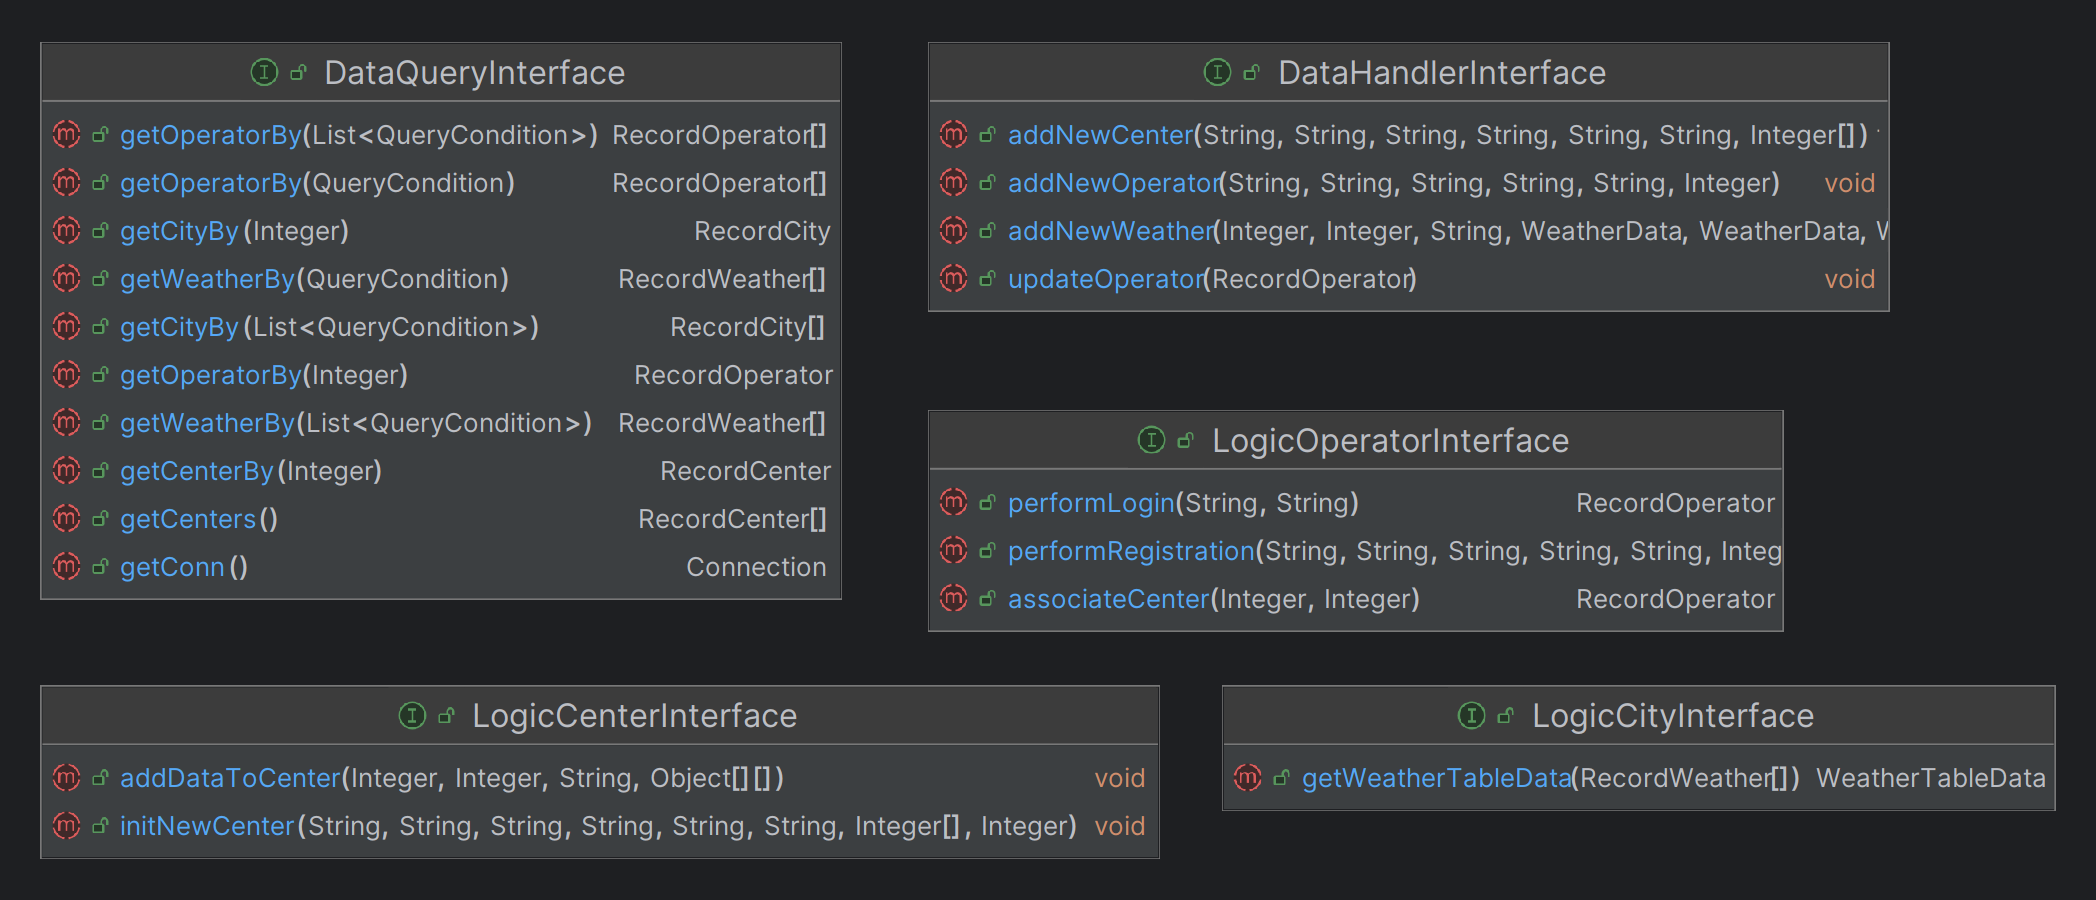
\includegraphics[scale = 0.2]{img/interfaceRMIPackage.png}
    \caption{UML delle classi del package interfacesRMI}
    \label{fig:InterfacesRMI}
\end{figure}

\subsubsection{DataHandlerInterface}
L'interfaccia \texttt{DataHandlerInterface} è un'interfaccia che permette di definire i metodi remoti che possono
essere invocati da un client per interagire con il server per la gestione dei dati.
Quest'interfaccia dev'essere implementata dalla classe \texttt{DataHandlerImp} la quale esegue i metodi dichiarati.
I metodi di tale interfaccia sono:
\begin{itemize}
    \item \texttt{void addNewOperator(String nameSurname, String taxCode, String email, String username, String password, Integer centerID)}
    \item \texttt{RecordCenter addNewCenter(String centerName, String streetName, String streetNumber, String CAP, String townName, String districtName, Integer[] cityIDs)}
    \item \texttt{void addNewWeather(Integer cityID, Integer centerID, String date, RecordWeather.WeatherData wind, RecordWeather.WeatherData humidity, RecordWeather.WeatherData pressure, RecordWeather.WeatherData temperature, RecordWeather.WeatherData precipitation, RecordWeather.WeatherData glacierElevation, RecordWeather.WeatherData glacierMass)}
    \item \texttt{void updateOperator(RecordOperator operator)}
\end{itemize}

\subsubsection{DataQueryInterface}
L'interfaccia \texttt{DataQueryInterface} è un'interfaccia che permette di definire i metodi remoti che possono
essere invocati da un client per interagire con il server per la gestione dei dati.
Quest'interfaccia dev'essere implementata dalla classe \texttt{DataQueryImp} la quale esegue i metodi dichiarati.
I metodi di tale interfaccia sono:
\begin{itemize}
    \item \texttt{RecordCity getCityBy(Integer ID)}
    \item \texttt{RecordCity[] getCityBy(List<QueryCondition> conditions)}
    \item \texttt{RecordOperator getOperatorBy(Integer ID)}
    \item \texttt{RecordOperator[] getOperatorBy(QueryCondition condition)}
    \item \texttt{RecordOperator[] getOperatorBy(List<QueryCondition> conditions)}
    \item \texttt{RecordCenter getCenterBy(Integer ID)}
    \item \texttt{RecordCenter[] getCenters()}
    \item \texttt{RecordWeather[] getWeatherBy(QueryCondition condition)}
    \item \texttt{RecordWeather[] getWeatherBy(List<QueryCondition> conditions)}
    \item \texttt{Connection getConn()}
\end{itemize}

\subsubsection{LogicCenterInterface}
L'interfaccia \texttt{LogicCenterInterface} è un'interfaccia che permette di definire i metodi remoti che possono
essere invocati da un client per interagire con il server per la gestione dei centri di monitoraggio.
Quest'interfaccia dev'essere implementata dalla classe \texttt{LogicCenterImp} la quale esegue i metodi dichiarati.
I metodi di tale interfaccia sono:
\begin{itemize}
    \item \texttt{void initNewCenter(String centerName, String streetName, String streetNumber, String CAP, String townName, String districtName, Integer[] cityIDs, Integer operatorID)}
    \item \texttt{void addDataToCenter(Integer cityID, Integer operatorID, String date, Object[][] tableData)}
\end{itemize}

\subsubsection{LogicCityInterface}
L'interfaccia \texttt{LogicCityInterface} è utilizzata per esporre i metodi che permettono di ottenere i dati relativi alle città, in particolare i dati metereologici.
Quest'interfaccia dev'essere implementata dalla classe \texttt{LogicCityImp} la quale esegue i metodi dichiarati.
I metodi di tale interfaccia sono:
\begin{itemize}
    \item \texttt{LogicCityImp.WeatherTableData getWeatherTableData(RecordWeather[] weatherRecords)}
\end{itemize}

\subsubsection{LogicOperatorInterface}
L'interfaccia \texttt{LogicOperatorInterface} è un'interfaccia che permette di definire i metodi remoti che possono essere invocati da un client per interagire con il server per la gestione della logica di business degli operatori.
Quest'interfaccia dev'essere implementata dalla classe \texttt{LogicOperatorImp} la quale esegue i metodi dichiarati.
I metodi di tale interfaccia sono:
\begin{itemize}
    \item \texttt{RecordOperator performLogin(String username, String password)}
    \item \texttt{void performRegistration(String nameSurname, String taxCode, String email, String username, String password, Integer centerID)}
    \item \texttt{RecordOperator associateCenter(Integer operatorID, Integer centerID)}
\end{itemize}

\subsection{Package record}
In questa sezione verranno descritti il package \texttt{record} e le classi che lo compongono.\\

\begin{figure}[H]
    \centering
    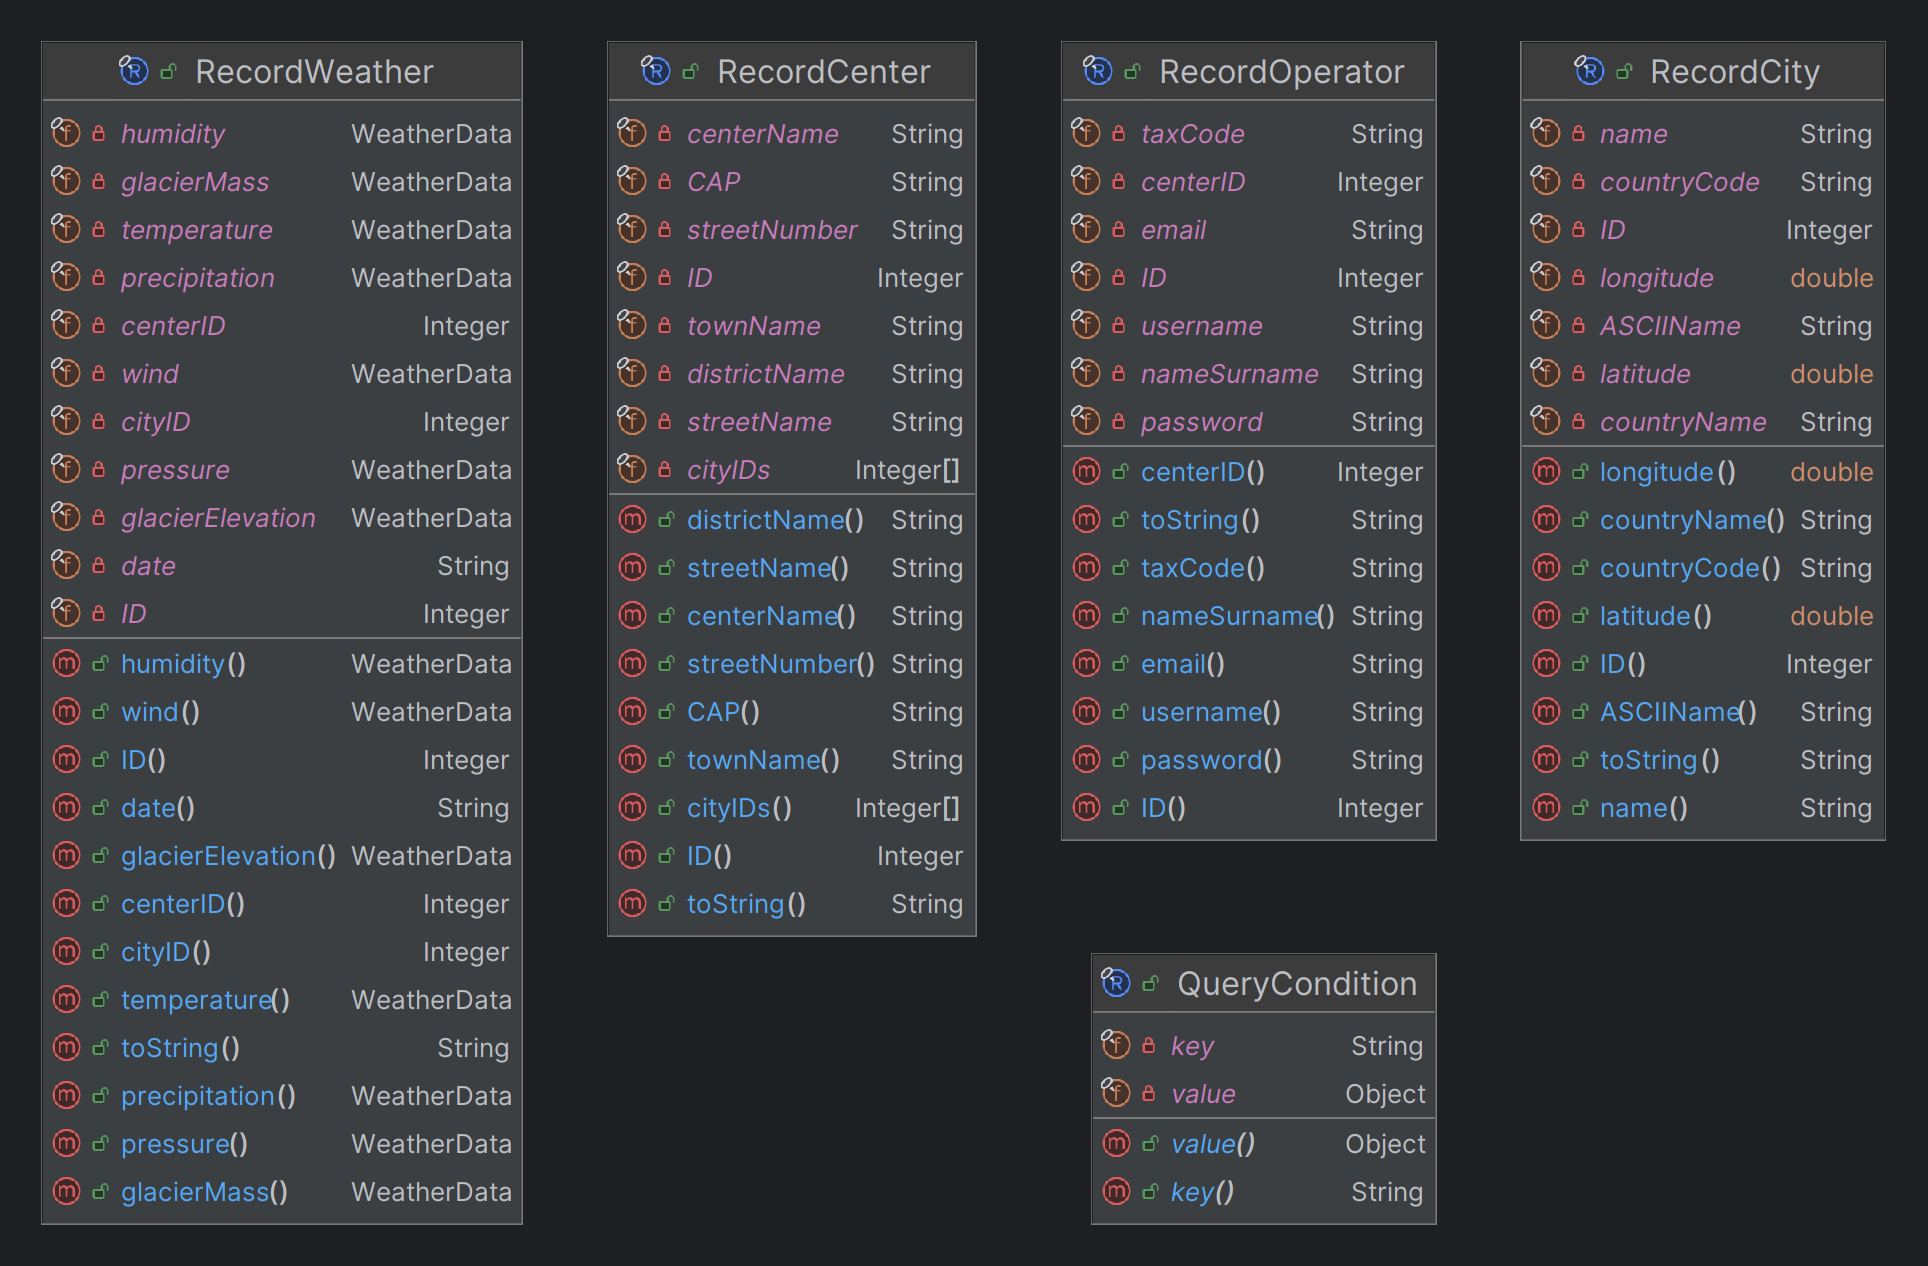
\includegraphics[scale = 0.2]{img/recordPackage.png}
    \caption{UML delle classi del package record}
    \label{fig:Record}
\end{figure}
\subsubsection{QueryCondition}
La classe \texttt{QueryCondition} rappresenta una condizione di query.\\
Viene utilizzata per definire una condizione di ricerca per i record presenti nel database.

\subsubsection{RecordCenter}
La classe \texttt{RecordCenter} rappresenta un centro di monitoraggio e contiene informazioni come il nome del centro, il nome della via, il numero civico, il CAP, il nome del comune, la sigla della provincia e una lista di ID delle città associate.
Questa classe è definita come un record, il che significa che è immutabile una volta creata.
I metodi di tale classe sono:
\begin{itemize}
    \item \texttt{public String toString()}
    \item \texttt{public Integer ID()}
    \item \texttt{public String centerName()}
    \item \texttt{public String streetName()}
    \item \texttt{public String streetNumber()}
    \item \texttt{public String CAP()}
    \item \texttt{public String townName()}
    \item \texttt{public String districtName()}
    \item \texttt{public String cityIDs()}
\end{itemize}

\subsubsection{RecordCity}
La classe \texttt{RecordCity} rappresenta una città e contiene informazioni come l'ID della città, il nome, il nome ASCII, il codice del paese, il nome del paese, la latitudine e la longitudine geografica.
Questa classe è definita come un record, il che significa che è immutabile una volta creata.
I metodi di tale classe sono:
\begin{itemize}
    \item \texttt{public String toString()}
    \item \texttt{public Integer ID()}
    \item \texttt{public String name()}
    \item \texttt{public String ASCIIname()}
    \item \texttt{public String countryCode()}
    \item \texttt{public String countryName()}
    \item \texttt{public double latitude()}
    \item \texttt{public double longitude()}
\end{itemize}

\subsubsection{RecordOperator}
La classe \texttt{RecordOperator} rappresenta un operatore e contiene informazioni come l'ID, il nome e cognome, il codice fiscale, l'email, il nome utente, la password e l'ID del centro di competenza (se assegnato).
Questa classe è definita come un record, il che significa che è immutabile una volta creata.
I metodi di tale classe sono:
\begin{itemize}
    \item \texttt{public String toString()}
    \item \texttt{public Integer ID()}
    \item \texttt{public String nameSurname()}
    \item \texttt{public String taxCode()}
    \item \texttt{public String email()}
    \item \texttt{public String username()}
    \item \texttt{public String password()}
    \item \texttt{public Integer centerID()}
\end{itemize}

\subsubsection{RecordWeather}
La classe \texttt{RecordWeather} rappresenta dati meteorologici registrati in una determinata data per una città e un centro specifici.
Questa classe contiene informazioni come l'ID, l'ID della città, l'ID del centro, la data e vari dati meteorologici come il vento, l'umidità, la pressione, la temperatura, la precipitazione, l'elevazione del ghiacciaio e la massa del ghiacciaio.
Questa classe è definita come un record, il che significa che è immutabile una volta creata.
I metodi di tale classe sono:
\begin{itemize}
    \item \texttt{public String toString()}
    \item \texttt{public Integer ID()}
    \item \texttt{public Integer cityID()}
    \item \texttt{public Integer centerID()}
    \item \texttt{public String date()}
    \item \texttt{public WeatherData wind()}
    \item \texttt{public WeatherData humidity()}
    \item \texttt{public WeatherData pressure()}
    \item \texttt{public WeatherData temperature()}
    \item \texttt{public WeatherData precipitation()}
    \item \texttt{public WeatherData glacierElevation()}
    \item \texttt{public WeatherData glacierMass()}
    \item \texttt{public Integer score()}
    \item \texttt{public String comment()}
\end{itemize}

\subsection{Package utils}
In questa sezione verranno descritti il package \texttt{utils} e le classi che lo compongono.\\

\begin{figure}[H]
    \centering
    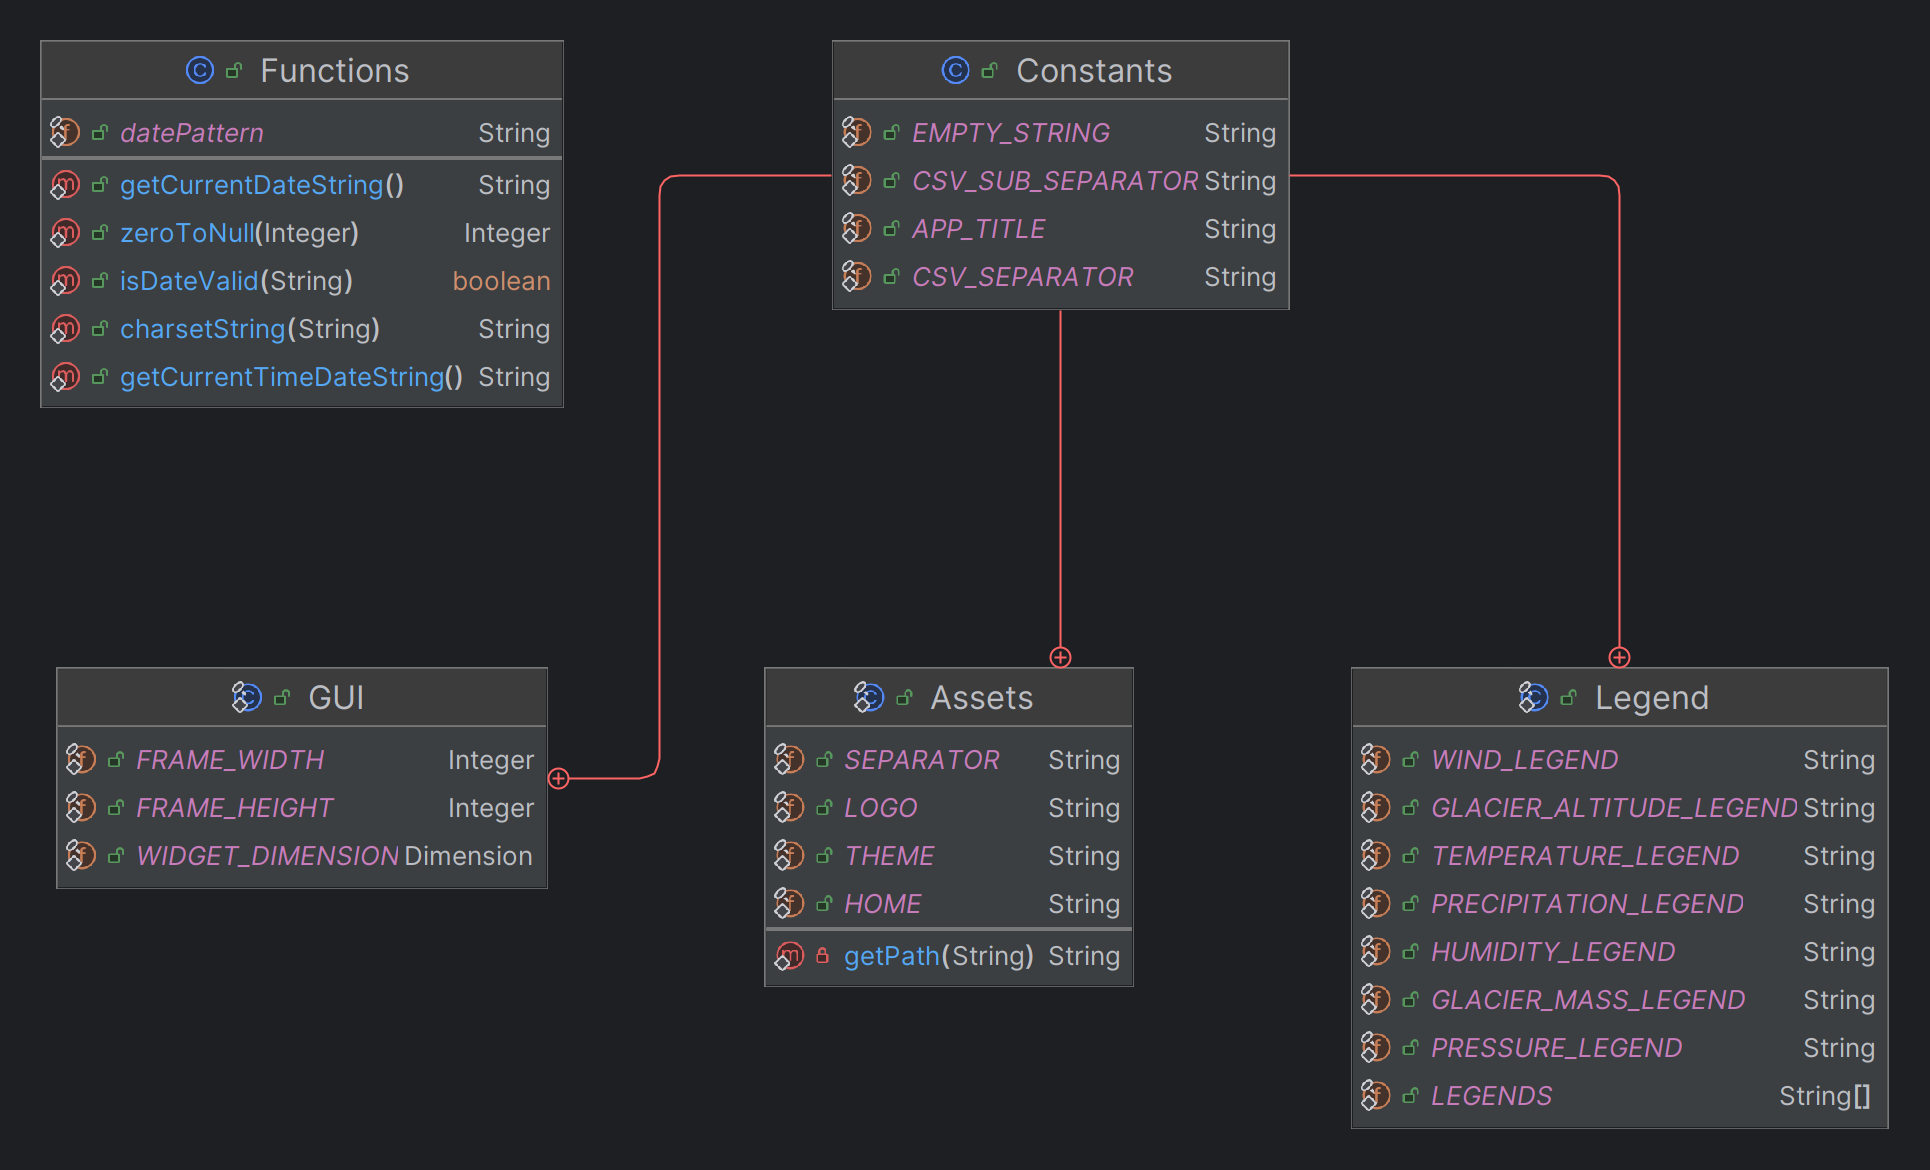
\includegraphics[scale = 0.2]{img/utils_1.png}
    \caption{UML delle classi Functions e Constants}
    \label{fig:Utils1}    
\end{figure}

\begin{figure}[H]
    \centering
    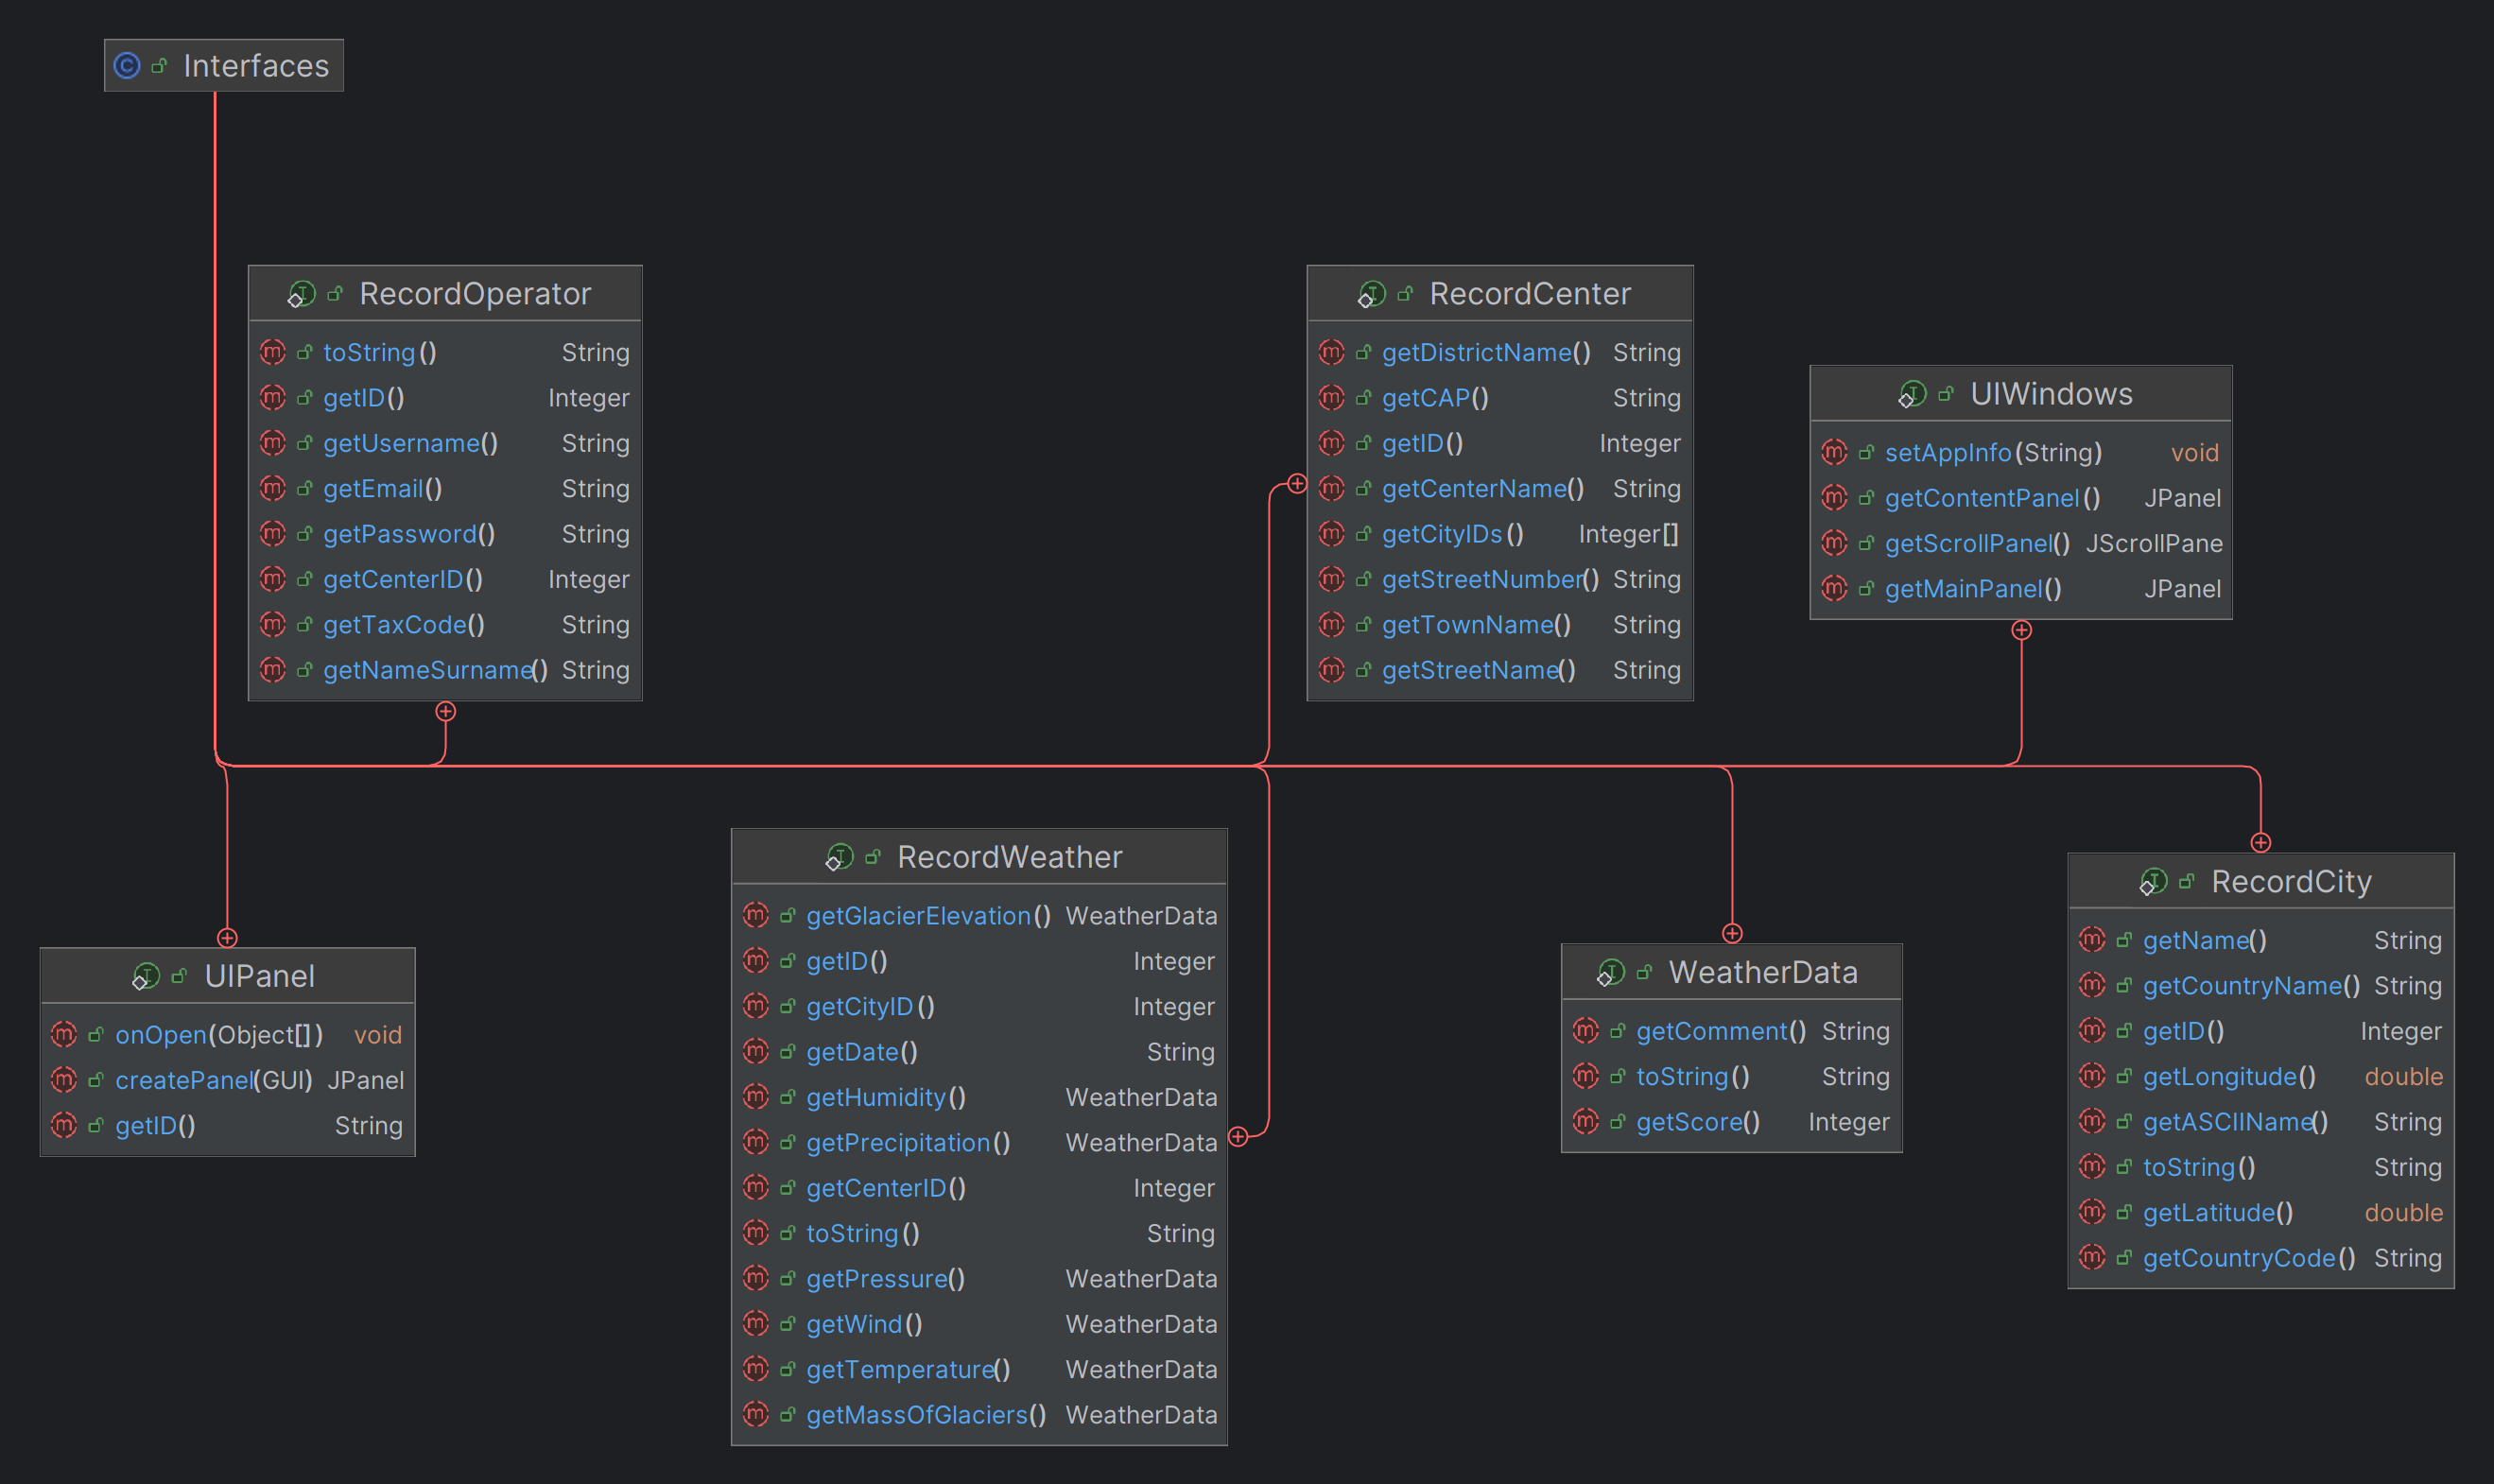
\includegraphics[scale = 0.1]{img/utils_2.png}
    \caption{UML delle classi Interfaces}
    \label{fig:Utils2}    
\end{figure}

\subsubsection{Constants}
La classe \texttt{Constants} fornisce una serie di costanti e definizioni utilizzate nell'applicazione.
Queste costanti includono separatori CSV, titolo dell'applicazione, indici di dati, percorsi dei file, dimensioni GUI predefinite e dati predefiniti.
La classe è progettata per memorizzare costanti utilizzate in tutto il codice e semplificare eventuali modifiche future.

\subsubsection{Functions}
La classe \texttt{Functions} fornisce una serie di funzioni di utilità per la gestione delle date e degli orari.
Queste funzioni includono la generazione della data corrente, la validazione delle date e la generazione della data e dell'orario correnti.
I metodi di tale classe sono:
\begin{itemize}
    \item \texttt{public static String getCurrentDateString()}: restituisce una stringa rappresentante la data corrente nel formato \textbf{yyyy-MM-dd}.
    \item \texttt{public static boolean isDateValid(String dateString)}: verifica se una stringa rappresentante una data è valida e non successiva alla data corrente.
    \item \texttt{public static String getCurrentTimeDateString()}: restituisce una stringa rappresentante la data e l'orario correnti nel formato \textbf{yyyy-MM-dd HH:mm:ss}.
    \item \texttt{public static String charsetString(String string)}: converte una stringa in un formato compatibile con il charset UTF-8.
    \item \texttt{public static Integer zeroToNull(Integer value)}: converte un valore 0 in un valore nullo.
\end{itemize}

\subsubsection{Interfaces}
L'interfaccia \texttt{Interfaces} definisce una serie di interfacce e contratti che rappresentano diversi aspetti ed entità all'interno del sistema.
Queste interfacce definiscono le proprietà e i metodi che devono essere implementati da classi specifiche per fornire funzionalità legate a città, operatori, centri, dati meteorologici, finestre UI e pannelli UI.
Per le interfacce dei record i metodi sono i getter degli attributi.
Invece per l'interfaccia di UI Windows i metodi sono:
\begin{itemize}
    \item \texttt{JPanel getMainPanel()}
    \item \texttt{JScrollPane getScrollPanel()}
    \item \texttt{JPanel getContentPanel()}
    \item \texttt{void setAppInfo(String text)}
\end{itemize}
Infine per l'interfaccia di UI Panel i metodi sono:
\begin{itemize}
    \item \texttt{JPanel createPanel(GUI gui)}
    \item \texttt{void onOpen(Object[] args)}
    \item \texttt{String getID()}
\end{itemize}

